% M.Sc. Dissertation Template
%	A work by Mário Cristóvão, based on an example by Gonçalo Martins and José Faria.

% Preamble
\documentclass[a4paper, 12pt]{report}

% Includes
\usepackage[usenames,dvipsnames]{xcolor}
\usepackage[utf8]{inputenc}				% UTF-8 encoding, so that you can use characters like ç and ã
\usepackage[T1]{fontenc}				% Same, but for output encoding
\usepackage[portuguese,english]{babel}	% Still related to the above
\setlength {\marginparwidth }{2cm}
\usepackage{todonotes}
\usepackage{acronym}					% List of acronyms
\usepackage{textcomp} 					% Extra characters
\usepackage{graphicx} 					% \includegraphics{}, the most common command to include images in figures 
\usepackage{titlesec}		 			% To manually format the chapter titles
\usepackage[left=3cm,right=2cm,top=2.5cm,bottom=2.5cm]{geometry} % Margins, as dictated by the rules
\usepackage[nottoc]{tocbibind} 	% Hyperlinks in table of contents, useful for navigation
\usepackage{multirow, makecell, pifont, rotating}
\usepackage[section]{placeins}			% \FloatBarrier, a useful command when your figures are trying to run away
\usepackage{caption}					% For captioning figures
\usepackage{subcaption}					% Subfigures (the subfigure package is deprecated and should not be used)
\usepackage[toc,page]{appendix}			% Appendices
\usepackage{pdfpages}					% Useful when your appendix is a pre-compiled PDF, such as a whole paper
\usepackage{url}						% Useful when one wants to include URLs in the text
\usepackage[
      colorlinks=true,    			%no frame around URL
      urlcolor=black,    			%no colors
      menucolor=black,    			%no colors
      linkcolor=black,    			%no colors
      citecolor=black,    			%no colors
      bookmarks=true,    			%tree-like TOC
      bookmarksopen=true,    		%expanded when starting
      bookmarksnumbered=true, 		%Put section numbers in bookmarks
      hyperfootnotes=true,    		%no referencing of footnotes, does not compile
      pdfpagemode=UseOutlines,    	%show the bookmarks when starting the pdf viewer
      plainpages=false, 			%solve problem ``destination with the same identifier'' warning
      pdfpagelabels				 	%solve problem ``destination with the same identifier'' warning
]{hyperref} 							% So that our citations look good and still work as links
\usepackage{epigraph}					% For your inspirational quote
\usepackage{etoolbox}
\usepackage{float}
\usepackage{arydshln}
\usepackage{tikz,lipsum,lmodern}
\usepackage[most]{tcolorbox}
\usepackage{graphicx}
\usepackage{listings}
\usepackage{lipsum}

\lstset{
    backgroundcolor=\color{backcolour},   
    commentstyle=\color{codegreen},
    keywordstyle=\color{magenta},
    numberstyle=\tiny\color{codegray},
    stringstyle=\color{codepurple},
    basicstyle=\linespread{0.8}\ttfamily\small,
    breakatwhitespace=false,         
    breaklines=true,                 
    captionpos=b,                    
    keepspaces=true,                 
    numbers=left,                    
    numbersep=5pt,                  
    showspaces=false,                
    showstringspaces=false,
    showtabs=false,                  
    tabsize=2
}

\renewcommand\cellalign{lc}
\newcommand{\xmark}{\ding{55}}%
\newcommand{\cmark}{\ding{51}}%
\setlength{\headheight}{16pt}
\renewcommand{\baselinestretch}{1.5}	% 1.5 line spacing, as mandated by the rules
\renewcommand{\familydefault}{\rmdefault}

\def\checkmark{\tikz\fill[scale=0.4](0,.35) -- (.25,0) -- (1,.7) -- (.25,.15) -- cycle;}

%---FORMAT CHAPTERS---

% Different Formating styles for the chapter, 
% uncomment your preferred style

% Simple Format
%\titleformat{\chapter}[hang]
%{
%  \sffamily
%  \Huge
%  \bfseries
%}
%{\thechapter}{0.5em}
%{}

% Line Format
\titleformat{\chapter}[hang]
{
  \sffamily
  \Huge
  \bfseries
}
{\thechapter}{0.5em}
{}
[\vspace{-3.0ex} \rule{\textwidth}{2pt}]

% Framed Format
%\titleformat{\chapter}[frame]
%{
%  \sffamily
%  \Huge
%  \bfseries
%}
%{Chapter \thechapter}{0.5em}
%{}


%---STYLE FOR CODE---

%Example of adding a new language (Julia in this case)
%\lstdefinelanguage{Julia}%
%  {morekeywords={abstract,break,case,catch,const,continue,do,else,elseif,%
%      end,export,false,for,function,immutable,import,importall,if,in,%
%      macro,module,otherwise,quote,return,switch,true,try,type,typealias,%
%      using,while},%
%   sensitive=true,%
%   alsoother={\$},%
%   morecomment=[l]\#,%
%   morecomment=[n]{\#=}{=\#},%
%   morestring=[s]{"}{"},%
%   morestring=[m]{'}{'},%
%}[keywords,comments,strings]%

\lstset{aboveskip=20pt,belowskip=20pt}
\definecolor{codegreen}{rgb}{0,0.3,0}
\definecolor{codegray}{rgb}{0.5,0.5,0.5}
\definecolor{codepurple}{rgb}{0.38,0,0.62}
\definecolor{backcolour}{rgb}{1,1,1}


\newcommand{\MONTH}{%
  \ifcase\the\month
  \or January% 1
  \or February% 2
  \or March% 3
  \or April% 4
  \or May% 5
  \or June% 6
  \or July% 7
  \or August% 8
  \or September% 9
  \or October% 10
  \or November% 11
  \or December% 12
  \fi}
\makeatletter
\newcommand{\YEAR}{\the\year}
\makeatother
\colorlet{shadecolor}{lightgray}

\newcommand{\thesistitle}{Design of a Multi-Sensor Apparatus for Forestry Robotics: A case study for Forest 3D Mapping}		% Your work's title
\newcommand{\myname}{Mário Cristóvão}				% Your name
\newcommand{\statedate}{Coimbra, \MONTH\ \YEAR}					% The date, usually "Place, Month Year"
\newcommand{\supervisorname}{David Portugal}		% Your supervisor's name
%\newcommand{\cosupervisorname}{co-supervisor 1 \linebreak co-supervisor 2}	% Your co-supervisor's name, if any.

% MAIN DOCUMENT
\begin{document}

\pagenumbering{roman}

% TITLE PAGES
% Uncomment this line when you have your cover ready. An MSWord template is available at that folder.
% You should edit it in MSWord, and then export it into PDF, so we can neatly import it here.
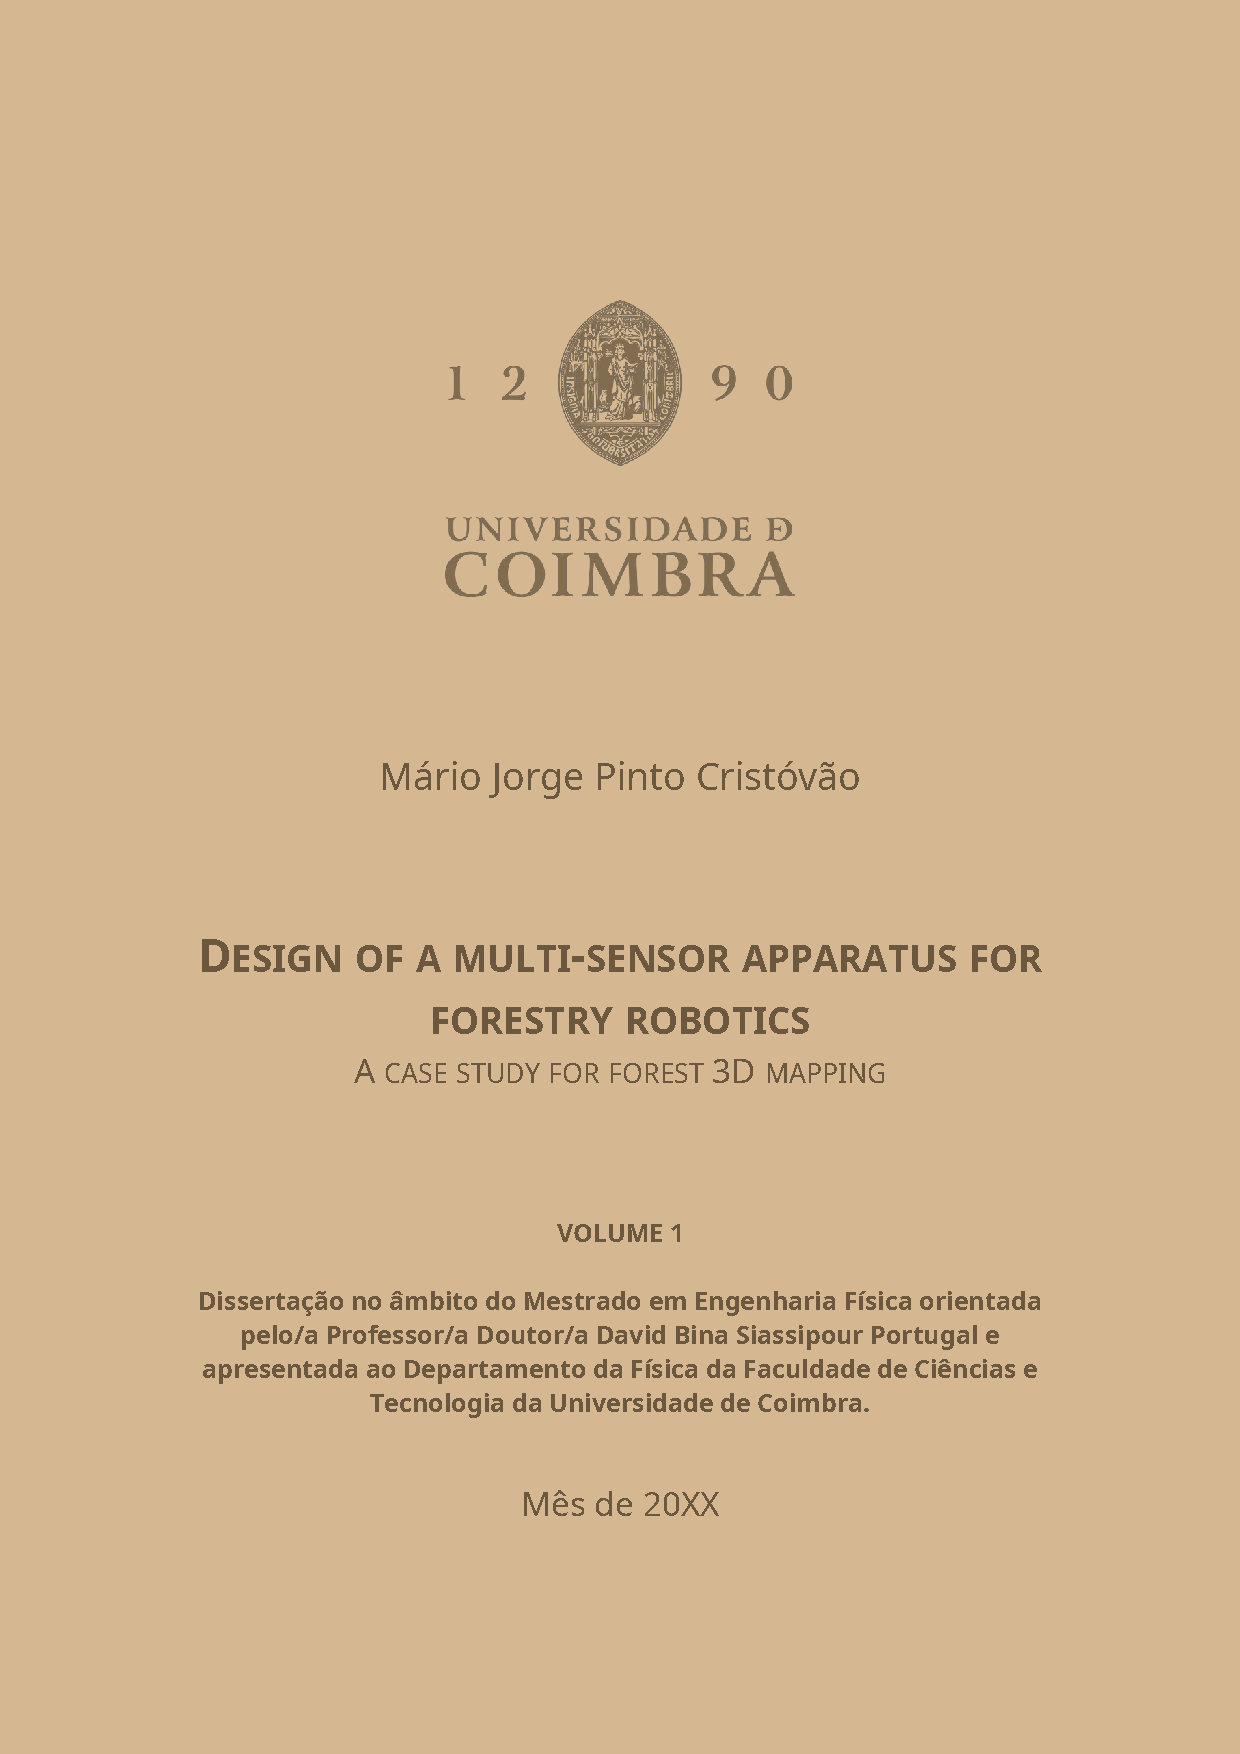
\includepdf[pages={-}]{images/cover.pdf}
% Blank page
%\newpage
%\thispagestyle{empty}
%\mbox{}
% Title page
\begin{titlepage}
    \begin{center}
    % UC logo, no name
    
\includegraphics[width=\textwidth]{images/FCTUC_H_FundoClaro.png}
    
    % Thesis name
    \vspace{1cm}
    {\huge{\textbf{\thesistitle}}\par}
    
    \vspace{1cm}
    {\large{\textbf{Supervisor:}\\\supervisorname\par}}
    \vspace{5mm}
    {\large{\textbf{Co-Supervisor:}\\\cosupervisorname}}
    
    \vspace{1cm}
    {\large{\textbf{Jury:}
    
    Prof. Jury1
    
    Prof. Jury2
    
    Prof. Jury3
    
    }}
    
    % Final Stuff
    \vfill
    Dissertation submitted in partial fulfillment for the degree of Master of Science in Engineering Physics.
    
    \vspace{0.5cm}
    {\large \statedate\par}    
    
    
    \end{center}
    \end{titlepage}
% Blank page
\newpage
\thispagestyle{empty}
\mbox{}

% Acknowledgements
\chapter*{Acknowledgments}
\addcontentsline{toc}{chapter}{Acknowledgements}
\lipsum[9]
% You can add blank pages here, if you like

% ABSTRACT
\chapter*{Resumo}
\addcontentsline{toc}{chapter}{Resumo}
\lipsum[4]
% And here

\chapter*{Abstract}
\addcontentsline{toc}{chapter}{Abstract}
\lipsum[4]
% And here as well
\newpage\null\thispagestyle{empty}\newpage

% INSPIRATIONAL QUOTE
% Setup
\setlength\epigraphwidth{12cm}
\setlength\epigraphrule{0pt}
\makeatletter
\patchcmd{\epigraph}{\@epitext{#1}}{\itshape\@epitext{#1}}{}{}
\makeatother
% Actual Quote
\vspace*{\fill}
\epigraph{"Intelligence is the ability to avoid doing work, yet getting the work done.”}
{Linus Torvald}
\vspace*{\fill}
\newpage\null\thispagestyle{empty}\newpage
% TABLE OF CONTENTS
\pagestyle{plain}
\tableofcontents
% LIST OF ACRONYMS
\chapter*{List of Acronyms}
\addcontentsline{toc}{chapter}{List of Acronyms}
\begin{acronym}[PROJECT\_NAME]
    \acro{DBH}{Diameter at Breast Height}
    \acro{EKF}{Extended Kalman Filter}
    \acro{FOV}{Field Of View}
    \acro{GNSS}{Global Navigation Satelite System}
    \acro{GPS}{Global Position System}
    \acro{ICP}{Iterative Closest Point}
    \acro{IFR}{Industrial Federation of Robotics}
    \acro{IMU}{Inertial Measurement Unit}
    \acro{LiDAR}{Laser imaging, Detection, and Ranging}
    \acro{LOAM}{\acs*{LiDAR} Odometry And Mapping}
    \acro{LIO-SAM}{\acs*{LiDAR} Inertial Odometry via Smoothing and Mapping}
    \acro{PDF}{Probability Dense Function}
    \acro{RMSE}{Root Mean Square Error}
    \acro{ROS}{Robot Operating System}
    \acro{SLAM}{Simultaneous Localization And Mapping}
    \acro{STD}{Standard Deviation}
    \acro{UKF}{Unscented Kalman Filter}
\end{acronym}
% LIST OF FIGURES
\listoffigures
% LIST OF TABLES
\listoftables
% BODY
\newpage
\thispagestyle{empty}
\mbox{}
\pagenumbering{arabic}	% Arabic numbering starts

% For each chapter, you should have a bit of code that looks like this:
% \label allows you to later \ref that chapter.
% \input includes a different .tex file, so that you can have you dissertation
% neatly partitioned into several files. I recommend one file per chapter.



%-----------------CHAPTERS--------------------

%-----CHAPTER1-INTRODUCTION-----
\chapter{Introduction}
\label{chap:introduction}
Due to their destructive nature, wildfires are often viewed as something to be avoided at all costs, however wildfires play a crucial role in a variety of ecosystems. In addition to rejuvenating the forest, wildfires can increase soil fertility and remove dead organic material, which decreases the likelihood of a more intense and destructive wildfire in the future \cite{bond_fires_2017}. In most fires, the problem occurs when they spiral out of control, causing unintended damage to wildlife and populations. Global warming and an increase in droughts have led to more frequent intensive wildfires in countries that were not historically prone to them. Throughout the Mediterranean region, countries have become accustomed to this natural destructive cycle and have been able to reduce burned areas since 1980 by improving fire control, Portugal remains the exception \cite{turco_decreasing_2016}, \cite{european_commission_joint_research_centre_forest_2021}. Keeping a forest clean is essential for controlling wildfires, and forest maintenance plays a crucial role in doing so. Like in other areas, bringing mechanization into the scope of forestry has greatly improve the productivity, leaving the human component as the bottleneck \cite{parker_robotics_2016}.

According to the \acl{IFR} (\acs{IFR}) report in 2020, the need for robotics is increasing every year  \cite{IFR_robot_report_2020}. Among the many uses of robots, there are healthcare applications, industrial application, agriculture, common households tasks like cleaning as well as dangerous or inaccessible tasks, such as space exploration and mining. It is only natural to assume that robots can play an active role in forestry applications. Although there is not a widespread use of forestry robots, some prototypes were already developed.  Some of these robots are designed to preserve and monitor forests \cite{couceiro_semfire_2019}, \cite{jelavic_towards_2021}, \cite{lam_flexible_2011}, \cite{notomista_slothbot_2019}, while others focus in actively fighting wildfires \cite{noauthor_firefighting_2014}  \cite{hose_cartridge}, \cite{hydra}. Furthermore, there are robots specialized in planting, pruning, and harvesting \cite{noauthor_multiscope_nodate}, \cite{molina_aerial_2017}, \cite{zhang_rubber-tapping_2019}.

Some of these robots weigh over a ton, have large dimensions, and lack flexibility. Consequently, this movement constraint leads to a slow acquisition of data causing a bottleneck in an engineering project's typical workflow: design, develop, test and repeat, since it results in unnecessary delays between the development and testing phases. This bottleneck can be alleviated by the use of a lightweight and portable system designed to gather data efficiently.

In short, wildfires are important to a healthy ecosystem but they need to be controlled to not damage populations and wildlife. The first step to increasing fire control is to clean the forest of dead organic matter, a task that can be performed by robots. As these robots are heavy, scientists and researchers find it difficult to obtain data directly from them, requiring a light system to record the necessary data to develop and test algorithms.

\section{Objectives}
In this work, we aim to design a rigid multisensory apparatus with an onboard computer to map forests. This apparatus combines multiple sensing technologies, such as 3D \acs{LiDAR}, depth cameras, infrared spectroscopy and \acl{IMU} (\acs{IMU}). With this apparatus, we will be able to collect datasets from forest environments, thus supporting forest operations, such as metric-semantic 3D mapping, combustible material identification, and forest cleaning. Aside from designing the apparatus, it is intended to integrate, test, and then compare state-of-the-art 3D mapping techniques based on the ROS middleware.

\section{System Requirements}

In order to create a system able to collect the necessary data while ensuring it complies with the requirements of future projects the MoSCoWW analysis was made and it is presented in Figure \ref{fig: moscoww}.

\begin{figure}[H]
    \centering
    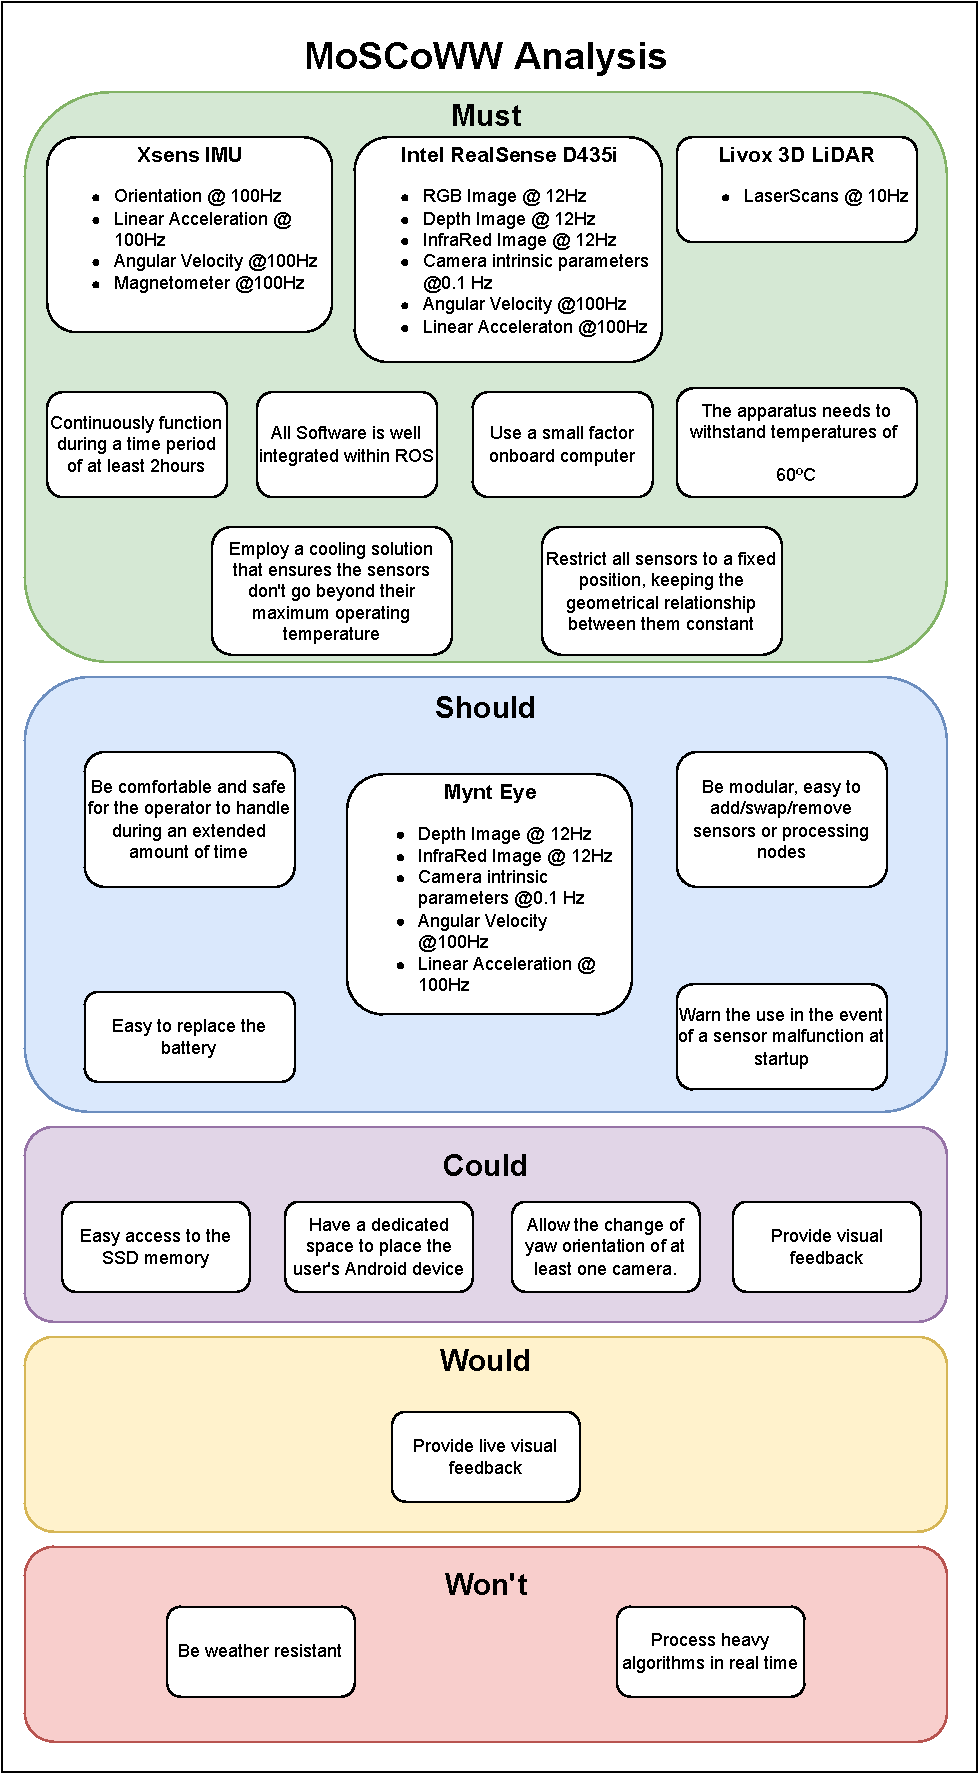
\includegraphics[width=0.875\linewidth]{images/introduction/moscoww_analysis.pdf}
    \caption{MoSCoWW analysis for the project}
    \label{fig: moscoww}
\end{figure}

\section{Dissertation Structure}

% Add your necessary chapters
\chapter{Background and Related Work}
\label{chap:background}
This chapter introduces and explains the fundamentals to understand the rest of the work presented in this disseration.

\section{\acl*{SLAM} (\acs*{SLAM})}

From the beginning of civilization, mapping the surroundings has been a key concept for navigating the environment. In essence we faced the same problem as our ancestors: How do we map the environment and know our location within it? \acs*{SLAM} is the challenge of mapping the local environment of a moving entity (e.g. robot) and updating the map continuously as the entity moves throughout space. This is a massive problem to tackle on and of extreme importance to achieve robot autonomy in moving robots. A common way to solve this problem is to use a Kalman filter.

The Kalman filter is an iterative process, as shown in Fig. \ref*{fig: flowchart kalman}, that uses consecutive data input to quickly converge to the true value. Each iteration involves computing three values: the Kalman gain, the current estimate, and its uncertainty. The Kalman gain uses the previous uncertainty and the error in data. The estimate of the current iteration is computed with the new data input and the previous estimation, where the weight of each component is decided by the kalman gain. Once the current estimate has been calculated, the new uncertainty of the estimate is computed with the current estimate and kalman gain.

\begin{figure}[H]
    \centering
    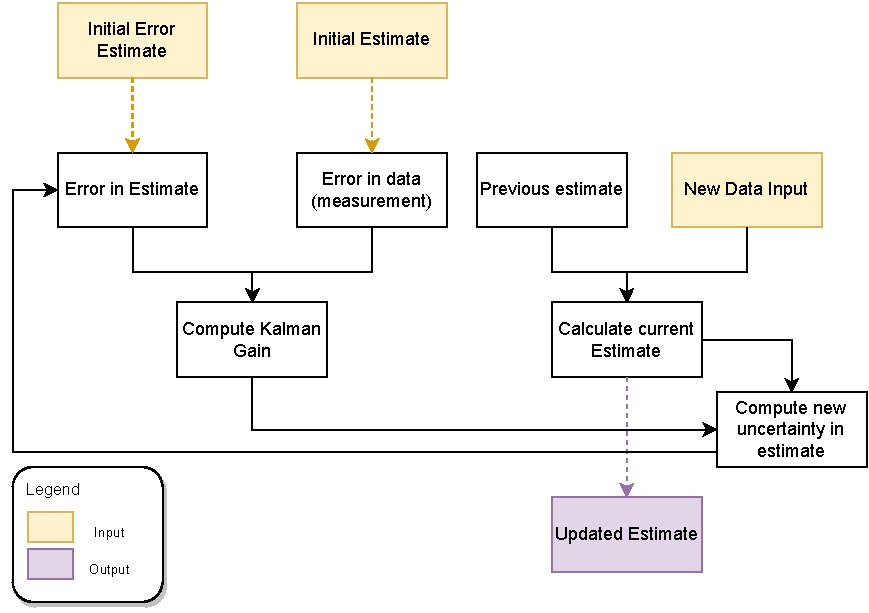
\includegraphics[width=0.7\linewidth]{images/background/Kalman-diagram.pdf}
    \caption{Flowchart of Kalman Filter. \textcolor{red}{ADD REFERENCE}}
    \label{fig: flowchart kalman}
\end{figure}

\subsection{Common sensors in \acs*{SLAM}}

\subsection{Loop Closure}

\subsection{Moving Objects}

\section{\acs{ROS}}

An effective robotics project cannot be achieved by just having sensors and physical components; rather, one must have a clever communication system between sensors and processes. Although such complex systems can be built from scratch, it is not worthwhile when software like \acs*{ROS} is available.

Although the name \acl*{ROS} suggests that ROS is an operating system, this is not the case.  In a way, \acs*{ROS} is both middleware and a framework. The system provides a communication channel where messages can be easily subscribed, published and distributed, allowing quick integration between systems and components. Moreover, it provides features such as debugging, visualization, testing, logging, and configuration right out of the box. Additionally, ROS includes a number of useful packages for essential areas relevant to robotics such as movement, perception, and manipulation. The ROS community is also constantly evolving with the most recent developments in robotics, so libraries are always being added to ROS. In robotics, it is considered the standard platform for developing complex projects.

% REFERENCES
% Edit the references.bib file to add your own references, that you can then
% \cite on your text.
\bibliographystyle{ieeetr}
\bibliography{bibliography/references.bib}
\titleformat{\chapter}[display]	% Return chapter titles to normal, taking up a whole page (cool for appendices)
{\normalfont\huge\bfseries}{\chaptertitlename\ \thechapter}{20pt}{\Huge}
%\begin{appendix}			% Start appendices
%\chapter{Sample Appendix}	% One chapter per appendix
%\label{app: sample appendix}
%\lipsum[5]
%\includepdf[pages={-}]{path/to/appendix.pdf}
% or
%\input{appendix_file}
%\end{appendix}
\end{document}